\documentclass{standalone}
\usepackage{graphicx}	
\usepackage{amssymb, amsmath}
\usepackage{color}

\usepackage{tikz}
\usetikzlibrary{intersections, backgrounds, math}
\usepackage{pgfmath}

\definecolor{light}{RGB}{220, 188, 188}
\definecolor{mid}{RGB}{185, 124, 124}
\definecolor{dark}{RGB}{143, 39, 39}
\definecolor{highlight}{RGB}{180, 31, 180}
\definecolor{light_teal}{RGB}{107, 142, 142}
\definecolor{mid_teal}{RGB}{72, 117, 117}
\definecolor{dark_teal}{RGB}{29, 79, 79}
\definecolor{gray10}{gray}{0.1}
\definecolor{gray20}{gray}{0.2}
\definecolor{gray30}{gray}{0.3}
\definecolor{gray40}{gray}{0.4}
\definecolor{gray60}{gray}{0.6}
\definecolor{gray70}{gray}{0.7}
\definecolor{gray80}{gray}{0.8}
\definecolor{gray90}{gray}{0.9}
\definecolor{gray95}{gray}{0.95}

\begin{document}

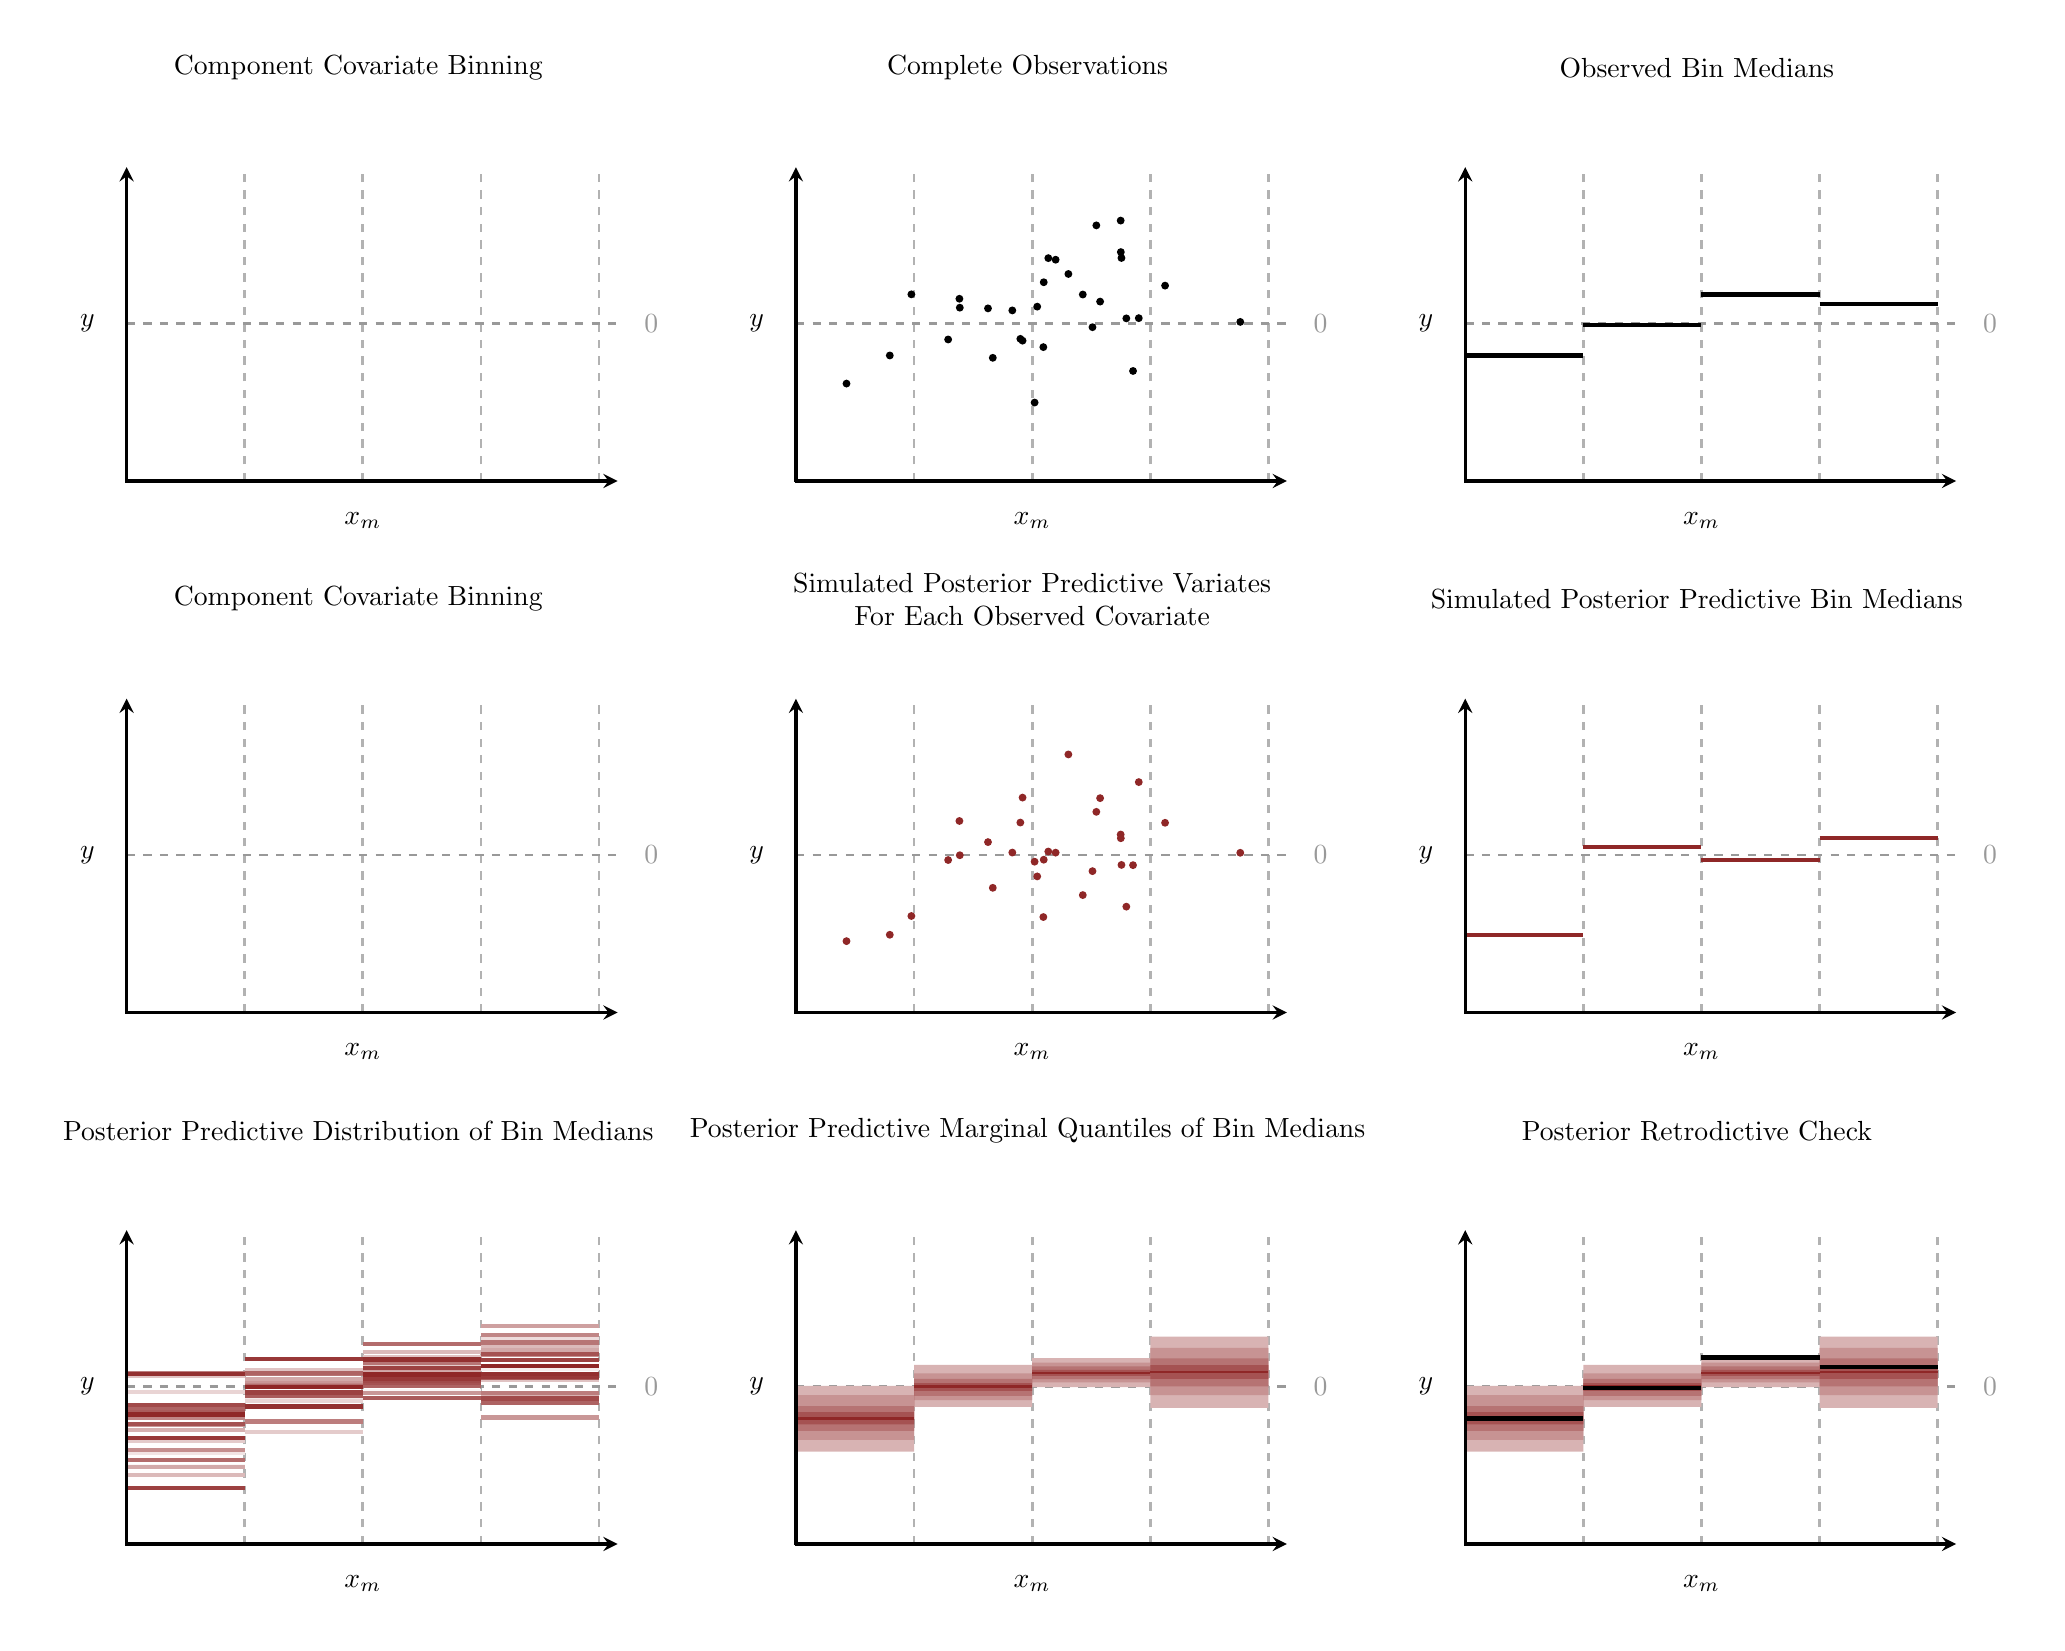
\begin{tikzpicture}[scale=1.0]

  \begin{scope}[shift={(0, 6.75)}]
    \draw[white] (-4.25, -3) rectangle (4.25, 3.75);
    
    \node[align=center] at (0, 3.25) { Component Covariate Binning };
    
    \foreach \b in {-3.0, -1.5,  0.0,  1.5,  3.0} {
      \draw[gray70, dashed, line width=1] (\b, -2) -- (\b, 2);
    }
    
    \draw[gray60, dashed, line width=1] (-3, 0) -- (3.25, 0);   
    \node[gray60, anchor=west] at (3.1, 0)  { $\quad 0$ };
     
    \draw [->, >=stealth, line width=1.25] (-3.00, -2.015) -- +(0, 4);
    \draw [->, >=stealth, line width=1.25] (-3.015, -2.00) -- +(6.25, 0);
    
    \node at (-3.5, 0) { $y$ };
    \node at (0, -2.5) { $x_{m}$ };
  \end{scope}
  
  \begin{scope}[shift={(8.5, 6.75)}]
    \draw[white] (-4.25, -3) rectangle (4.25, 3.75);
    
    \node[align=center] at (0, 3.25) { Complete Observations };
    
    \foreach \b in {-3.0, -1.5,  0.0,  1.5,  3.0} {
      \draw[gray70, dashed, line width=1] (\b, -2) -- (\b, 2);
    }
    
    \draw[gray60, dashed, line width=1] (-3, 0) -- (3.25, 0);   
    \node[gray60, anchor=west] at (3.1, 0)  { $\quad 0$ };
    
    \foreach \x/\mu in {0.205/0.830, 0.863/0.278, -0.150/-0.195, 0.142/-0.300, 0.147/0.524, 
                        1.354/0.068, -0.919/0.201, -0.561/0.192, 0.298/0.810, 1.134/0.832, 
                        -0.924/0.314, 0.064/0.214, -0.500/-0.436, 1.196/0.065, -0.122/-0.218, 
                        -2.358/-0.763, -0.252/0.166, 2.643/0.020, 1.281/-0.603, -1.808/-0.406, 
                        -1.067/-0.203, 1.688/0.481, 0.766/-0.047, 0.643/0.368, 0.031/-1.004, 
                        0.815/1.246, 0.460/0.629, -1.534/0.370, 1.126/0.907, 1.124/1.307} {
       \fill[black] (\x, \mu) circle(0.05);
    }
     
    \draw [->, >=stealth, line width=1.25] (-3.00, -2.015) -- +(0, 4);
    \draw [->, >=stealth, line width=1.25] (-3.015, -2.00) -- +(6.25, 0);
    
    \node at (-3.5, 0) { $y$ };
    \node at (0, -2.5) { $x_{m}$ };
  \end{scope}
  
  \begin{scope}[shift={(17, 6.75)}]
    \draw[white] (-4.25, -3) rectangle (4.25, 3.75);
    
    \node[align=center] at (0, 3.25) { Observed Bin Medians };
    
    \foreach \b in {-3.0, -1.5,  0.0,  1.5,  3.0} {
      \draw[gray70, dashed, line width=1] (\b, -2) -- (\b, 2);
    }
    
    \draw[gray60, dashed, line width=1] (-3, 0) -- (3.25, 0);   
    \node[gray60, anchor=west] at (3.1, 0)  { $\quad 0$ };
    
    \foreach \l/\r/\m in {-3.000/-1.500/-0.406, -1.500/0.000/-0.015, 
                          0.000/1.500/0.368, 1.500/3.000/0.250} {
       \draw[black, line width=1.5] (\l, \m) -- (\r, \m);
    }
     
    \draw [->, >=stealth, line width=1.25] (-3.00, -2.015) -- +(0, 4);
    \draw [->, >=stealth, line width=1.25] (-3.015, -2.00) -- +(6.25, 0);
    
    \node at (-3.5, 0) { $y$ };
    \node at (0, -2.5) { $x_{m}$ };
  \end{scope}

  \begin{scope}[shift={(0, 0)}]
    \draw[white] (-4.25, -3) rectangle (4.25, 3.75);
    
    \node[align=center] at (0, 3.25) { Component Covariate Binning };
    
    \foreach \b in {-3.0, -1.5,  0.0,  1.5,  3.0} {
      \draw[gray70, dashed, line width=1] (\b, -2) -- (\b, 2);
    }
    
    \draw[gray60, dashed, line width=1] (-3, 0) -- (3.25, 0);   
    \node[gray60, anchor=west] at (3.1, 0)  { $\quad 0$ };
     
    \draw [->, >=stealth, line width=1.25] (-3.00, -2.015) -- +(0, 4);
    \draw [->, >=stealth, line width=1.25] (-3.015, -2.00) -- +(6.25, 0);
    
    \node at (-3.5, 0) { $y$ };
    \node at (0, -2.5) { $x_{m}$ };
  \end{scope}
  
  \begin{scope}[shift={(8.5, 0)}]
    \draw[white] (-4.25, -3) rectangle (4.25, 3.75);
    
    \node[align=center] at (0, 3.25) { Simulated Posterior Predictive Variates\\For Each Observed Covariate };
    
    \foreach \b in {-3.0, -1.5,  0.0,  1.5,  3.0} {
      \draw[gray70, dashed, line width=1] (\b, -2) -- (\b, 2);
    }
    
    \draw[gray60, dashed, line width=1] (-3, 0) -- (3.25, 0);   
    \node[gray60, anchor=west] at (3.1, 0)  { $\quad 0$ };
    
    \foreach \x/\mu in {0.205/0.044, 0.863/0.722, -0.150/0.412, 0.142/-0.788, 0.147/-0.060, 
                        1.354/0.926, -0.919/-0.003, -0.561/0.164, 0.298/0.030, 1.134/-0.126, 
                        -0.924/0.432, 0.064/-0.272, -0.500/-0.417, 1.196/-0.656, -0.122/0.729, 
                        -2.358/-1.094, -0.252/0.031, 2.643/0.028, 1.281/-0.129, -1.808/-1.013, 
                        -1.067/-0.064, 1.688/0.409, 0.766/-0.205, 0.643/-0.509, 0.031/-0.085, 
                        0.815/0.548, 0.460/1.277, -1.534/-0.775, 1.126/0.213, 1.124/0.260} {
       \fill[dark] (\x, \mu) circle(0.05);
    }
     
    \draw [->, >=stealth, line width=1.25] (-3.00, -2.015) -- +(0, 4);
    \draw [->, >=stealth, line width=1.25] (-3.015, -2.00) -- +(6.25, 0);
    
    \node at (-3.5, 0) { $y$ };
    \node at (0, -2.5) { $x_{m}$ };
  \end{scope}
  
  \begin{scope}[shift={(17, 0)}]
    \draw[white] (-4.25, -3) rectangle (4.25, 3.75);
    
    \node[align=center] at (0, 3.25) { Simulated Posterior Predictive Bin Medians };
    
    \foreach \b in {-3.0, -1.5,  0.0,  1.5,  3.0} {
      \draw[gray70, dashed, line width=1] (\b, -2) -- (\b, 2);
    }
    
    \draw[gray60, dashed, line width=1] (-3, 0) -- (3.25, 0);   
    \node[gray60, anchor=west] at (3.1, 0)  { $\quad 0$ };
    
    \foreach \l/\r/\m in {-3.000/-1.500/-1.013, -1.500/0.000/0.098, 
                          0.000/1.500/-0.060, 1.500/3.000/0.218} {
       \draw[dark, line width=1.5] (\l, \m) -- (\r, \m);
    }
     
    \draw [->, >=stealth, line width=1.25] (-3.00, -2.015) -- +(0, 4);
    \draw [->, >=stealth, line width=1.25] (-3.015, -2.00) -- +(6.25, 0);
    
    \node at (-3.5, 0) { $y$ };
    \node at (0, -2.5) { $x_{m}$ };
  \end{scope}
  
  \begin{scope}[shift={(0, -6.75)}]
    \draw[white] (-4.25, -3) rectangle (4.25, 3.75);
    
    \node[align=center] at (0, 3.25) { Posterior Predictive Distribution of Bin Medians };
    
    \foreach \b in {-3.0, -1.5,  0.0,  1.5,  3.0} {
      \draw[gray70, dashed, line width=1] (\b, -2) -- (\b, 2);
    }
    
    \draw[gray60, dashed, line width=1] (-3, 0) -- (3.25, 0);   
    \node[gray60, anchor=west] at (3.1, 0)  { $\quad 0$ };
    
    \foreach \a/\b/\c/\d [count=\n] in {-1.013/0.098/-0.060/0.218, -0.247/-0.104/0.296/0.218,
                                        -0.848/-0.128/0.331/-0.128, -0.331/0.036/0.189/0.610, 
                                        -0.075/-0.182/0.299/-0.141, -0.697/-0.582/0.276/-0.190, 
                                        0.128/0.205/0.379/0.085, -1.120/-0.117/0.441/0.499, 
                                        -0.548/0.031/0.140/-0.139, -1.021/0.094/0.193/0.458, 
                                        -0.381/0.160/0.217/0.765, -0.487/0.042/-0.086/-0.393, 
                                        -0.811/-0.010/0.121/0.397, -0.399/0.021/0.084/0.653, 
                                        0.168/-0.445/0.086/-0.080, -0.240/0.156/0.298/0.558, 
                                        -0.936/0.002/0.540/-0.176, -0.291/0.172/0.010/-0.203, 
                                        -0.322/-0.124/-0.146/0.109, -0.481/0.349/0.046/0.408, 
                                        -0.240/-0.263/0.072/-0.152, -1.290/-0.077/0.233/0.337, 
                                        -0.656/0.349/0.096/0.123, 0.156/-0.254/0.343/0.162, 
                                        -0.355/-0.005/0.153/0.262} {
       \pgfmathsetmacro{\prop}{4 * \n};
       \colorlet{custom}{dark!\prop!white};
       \draw[custom, line width=1.5] (-3, \a)   -- (-1.5, \a);
       \draw[custom, line width=1.5] (-1.5, \b) -- (0, \b);
       \draw[custom, line width=1.5] (0, \c)    -- (1.5, \c);
       \draw[custom, line width=1.5] (1.5, \d)  -- (3, \d);
    }
     
    \draw [->, >=stealth, line width=1.25] (-3.00, -2.015) -- +(0, 4);
    \draw [->, >=stealth, line width=1.25] (-3.015, -2.00) -- +(6.25, 0);
    
    \node at (-3.5, 0) { $y$ };
    \node at (0, -2.5) { $x_{m}$ };
  \end{scope}
  
  \begin{scope}[shift={(8.5, -6.75)}]
    \draw[white] (-4.25, -3) rectangle (4.25, 3.75);
    
    \node[align=center] at (0, 3.25) { Posterior Predictive Marginal Quantiles of Bin Medians };
    
    \foreach \b in {-3.0, -1.5,  0.0,  1.5,  3.0} {
      \draw[gray70, dashed, line width=1] (\b, -2) -- (\b, 2);
    }
    
    \draw[gray60, dashed, line width=1] (-3, 0) -- (3.25, 0);   
    \node[gray60, anchor=west] at (3.1, 0)  { $\quad 0$ };
    
    \foreach \a/\b/\c/\d/\e/\f/\g/\h [count=\n] in {-0.827/-0.260/-0.009/-0.271/0.634/0.360/0.274/0.008, 
                                                    -0.679/-0.174/0.052/-0.109/0.489/0.304/0.168/-0.109, 
                                                    -0.563/-0.119/0.094/0.002/0.358/0.254/0.097/-0.249, 
                                                    -0.480/-0.057/0.136/0.098/0.270/0.212/0.042/-0.327} {
       \pgfmathsetmacro{\prop}{20 + 15 * \n};
       \colorlet{custom}{dark!\prop!white};
       \fill[custom] (-3, \a) -- (-1.5, \a) --
                     (-1.5, \b) -- (0, \b) --
                     (0, \c) -- (1.5, \c) --
                     (1.5, \d) -- (3, \d) --
                     (3, \e) -- (1.5, \e) --
                     (1.5, \f) -- (0, \f) --
                     (0, \g) -- (-1.5, \g) --
                     (-1.5, \h) -- (-3, \h) -- cycle;
    }
    
    \foreach \a/\b/\c/\d in {-0.40223321/-0.00139444/0.17260304/0.18371216} {
      \draw[dark, line width=1] (-3, \a) -- (-1.5, \a);
      \draw[dark, line width=1] (-1.5, \b) -- (0, \b);
      \draw[dark, line width=1] (0, \c) -- (1.5, \c);
      \draw[dark, line width=1] (1.5, \d) -- (3, \d);
    }
     
    \draw [->, >=stealth, line width=1.25] (-3.00, -2.015) -- +(0, 4);
    \draw [->, >=stealth, line width=1.25] (-3.015, -2.00) -- +(6.25, 0);
    
    \node at (-3.5, 0) { $y$ };
    \node at (0, -2.5) { $x_{m}$ };
  \end{scope}
  
  \begin{scope}[shift={(17, -6.75)}]
    \draw[white] (-4.25, -3) rectangle (4.25, 3.75);
    
    \node[align=center] at (0, 3.25) { Posterior Retrodictive Check };
    
    \foreach \b in {-3.0, -1.5,  0.0,  1.5,  3.0} {
      \draw[gray70, dashed, line width=1] (\b, -2) -- (\b, 2);
    }
    
    \draw[gray60, dashed, line width=1] (-3, 0) -- (3.25, 0);   
    \node[gray60, anchor=west] at (3.1, 0)  { $\quad 0$ };
    
    \foreach \a/\b/\c/\d/\e/\f/\g/\h [count=\n] in {-0.827/-0.260/-0.009/-0.271/0.634/0.360/0.274/0.008, 
                                                    -0.679/-0.174/0.052/-0.109/0.489/0.304/0.168/-0.109, 
                                                    -0.563/-0.119/0.094/0.002/0.358/0.254/0.097/-0.249, 
                                                    -0.480/-0.057/0.136/0.098/0.270/0.212/0.042/-0.327} {
       \pgfmathsetmacro{\prop}{20 + 15 * \n};
       \colorlet{custom}{dark!\prop!white};
       \fill[custom] (-3, \a) -- (-1.5, \a) --
                     (-1.5, \b) -- (0, \b) --
                     (0, \c) -- (1.5, \c) --
                     (1.5, \d) -- (3, \d) --
                     (3, \e) -- (1.5, \e) --
                     (1.5, \f) -- (0, \f) --
                     (0, \g) -- (-1.5, \g) --
                     (-1.5, \h) -- (-3, \h) -- cycle;
    }
    
    \foreach \a/\b/\c/\d in {-0.40223321/-0.00139444/0.17260304/0.18371216} {
      \draw[dark, line width=1] (-3, \a) -- (-1.5, \a);
      \draw[dark, line width=1] (-1.5, \b) -- (0, \b);
      \draw[dark, line width=1] (0, \c) -- (1.5, \c);
      \draw[dark, line width=1] (1.5, \d) -- (3, \d);
    }
    
    \foreach \l/\r/\m in {-3.000/-1.500/-0.406, -1.500/0.000/-0.015, 
                          0.000/1.500/0.368, 1.500/3.000/0.250} {
      \draw[black, line width=1.5] (\l, \m) -- (\r, \m);
    }
     
    \draw [->, >=stealth, line width=1.25] (-3.00, -2.015) -- +(0, 4);
    \draw [->, >=stealth, line width=1.25] (-3.015, -2.00) -- +(6.25, 0);
    
    \node at (-3.5, 0) { $y$ };
    \node at (0, -2.5) { $x_{m}$ };
  \end{scope}
  
  
\end{tikzpicture}

\end{document}  